\documentclass[a4paper,12pt]{article}
%%%%%%%%%%%%%%%%%%%%%%%%%%%%%%%%%%%%%%%%%%%%%%%%%%%%%%%%%%%%%%%%%%%%%%%%%%%%%%%%%%%%%%%%%%%%%%%%%%%%%%%%%%%%%%%%%%%%%%%%%%%%%%%%%%%%%%%%%%%%%%%%%%%%%%%%%%%%%%%%%%%%%%%%%%%%%%%%%%%%%%%%%%%%%%%%%%%%%%%%%%%%%%%%%%%%%%%%%%%%%%%%%%%%%%%%%%%%%%%%%%%%%%%%%%%%
\usepackage{eurosym}
\usepackage{vmargin}
\usepackage{amsmath}
\usepackage{graphics}
\usepackage{epsfig}
\usepackage{subfigure}
\usepackage{fancyhdr}
\usepackage{listings}
\usepackage{framed}
\usepackage{graphicx}
\usepackage{amsmath}
\usepackage{chngpage}
%\usepackage{bigints}

\setcounter{MaxMatrixCols}{10}

\begin{document}
%========================================================================%
\section{Plotting}
\begin{itemize}
\item Plotting is an intermediate-level interface that is centered around composing visual glyphs. 
\item Here, you create a visualization by combining various visual elements (dot, circles, line, patch and many others) 
and tools (hover tool, zoom, Save, reset and others).

\item Bokeh plots created using the \texttt{bokeh.plotting} interface comes with a default set of tools and visual styles. 
\end{itemize}
%=================================== %
\newpage
\subsection{Set Up}
For plotting, follow the below steps:

\begin{itemize}
\item Import library, methods or functions \\ ( something like ``\texttt{from bokeh.XXX import WWW, YYY, ZZZ} ")
\item Select the output mode (notebook, web browser, server) \\ (commands are \texttt{output\_file}, \texttt{output\_notebook} etc...)
\item Activate a figure ( call it \texttt{p})
\item Perform subsequent plotting operations, it will affect the generated figure.
\item Visualize it
\end{itemize}

\begin{framed}
	\begin{verbatim}
	
	### 1. Import all required utilities
	
	from bokeh.charts import Scatter, output_file, show
	from bokeh.sampledata.autompg import autompg as df
	
	
	### 2. Render the plot
	
	p = Scatter(df, x='displ', y='hp', marker='cyl', color='cyl',
	title="HP vs DISPL (marked by CYL)", legend="top_left",
	xlabel="Displacement", ylabel="Horsepower")
	
	
	### 3.  Output the plot as html
	
	output_file("scatter.html")
	
	 # output_notebook() as alternative
	
	### 4. Present the plot to screen
	
	show(p)
	
	\end{verbatim}
\end{framed}
\newpage

To understand these steps better, let me demonstrate these steps using examples below:


%========================================================================%
 
\newpage
\subsection{Plot Example-1} 

Create a scatter square mark on XY frame of notebook

\begin{framed}
\begin{verbatim}
from bokeh.plotting import figure, output_notebook, show

# output to notebook
output_notebook()
p = figure(plot_width=400, plot_height=400)

# add square with a size, color, and alpha
p.square([2, 5, 6, 4], [2, 3, 2, 1, 2], size=20, color="navy")

# show the results
show(p)

\end{verbatim}
\end{framed}
\begin{figure}[h!]
\centering
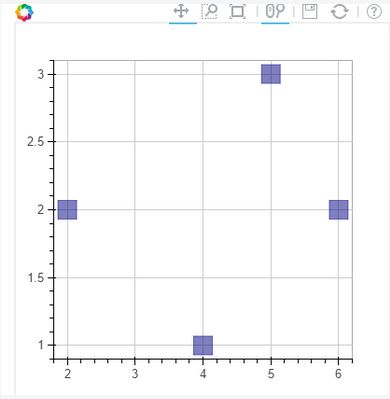
\includegraphics[width=0.7\linewidth]{images/02-plotting-AV-scatterplot}
\caption{}
\label{fig:02-plotting-AV-scatterplot}
\end{figure}

% %\subsection{Bokeh\_Scatter}
Similarly, you can create various other plots like line, wedges, arc, ovals, images, patches and many others, refer this link to see various example.


%========================================================================%
\newpage

\subsection{Plot Example-2: Combine two visual elements in a plot}
\begin{framed}
	\begin{verbatim}
from bokeh.plotting import figure, output_notebook, show

# output to notebook
output_notebook()

p = figure(plot_width=400, plot_height=400)

# add square with a size, color, and alpha
p.square([2, 5, 6, 4], [2, 3, 2, 1, 2], size=20, color="navy")

#added a line plot to existing figure
p.line([1, 2, 3, 4, 5], [1, 2, 2, 4, 5], line_width=2) 

# show the results
show(p)
\end{verbatim}
\end{framed}

%Multiple_Plots
\begin{figure}[h!]
\centering
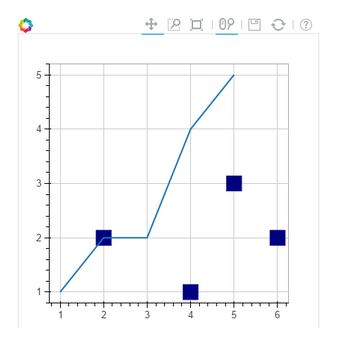
\includegraphics[width=0.7\linewidth]{images/02-plotting-AV-scatterplot-Line}
\caption{}
\label{fig:02-plotting-AV-scatterplot-Line}
\end{figure}


%========================================================================%
\newpage
\subsection{Plot Example-3: Add a hover tool and axis labels to above plot}
\begin{framed}
	\begin{verbatim}
from bokeh.plotting import figure, output_notebook, show
from bokeh.models import HoverTool, BoxSelectTool 
#For enabling tools

# output to notebook
output_notebook()

#Add tools
TOOLS = [BoxSelectTool(), HoverTool()]

p = figure(plot_width=400, plot_height=400, tools=TOOLS)

# add a square with a size, color, and alpha
p.square([2, 5, 6, 4], [2, 3, 2, 1, 2], size=20, color="navy", alpha=0.5)

#Visual Elements
p.xaxis.axis_label = "X-axis"
p.yaxis.axis_label = "Y-axis"

# show the results
show(p)
\end{verbatim}
\end{framed}

%Bokeh_Tools_Visualize
\begin{figure}[h!]
\centering
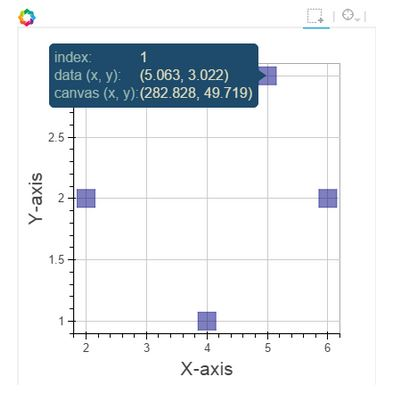
\includegraphics[width=0.5\linewidth]{images/02-plotting-AV-scatterplot-interactive}
\caption{}
\label{fig:02-plotting-AV-scatterplot-interactive}
\end{figure}

For more details on visual attributes and tools refer these links:

Styling visual attributes
Configuring plot tools
 
%========================================================================%

%Plot Example-4: Plot map of India using latitude and longitude data for boundaries
%


%
%
%Note: I have data for polygon of latitude and longitude for boundaries of India in a csv format. I will use that for plotting.
%
%Here, we will go with patch plotting, let’s look at the commands below:
%
%#Import libraries
%import pandas as pd
%from bokeh.plotting import figure, show, output_notebook
%#Import Latitude and lanogitude co-ordinates
%India=pd.read_csv('E:/India.csv')
%del India['ID']
%India.index=['IN0','IN1','IN2','IN3','IN4','IN5']
%#Convert string values to float as co-ordinates in dataframe are string
%for j in range(0,len(India)):
% a = India['lats'][j]
% India['lats'][j] = [float(i) for i in a[1:len(a)-1].split(",")]
%for j in range(0,len(India)):
% a = India['lons'][j]
% India['lons'][j] = [float(i) for i in a[1:len(a)-1].split(",")]
%# Output option
%output_notebook()
%# Create your plot
%p = figure(plot_height=400, plot_width=400, toolbar_location="right",x_axis_type=None, y_axis_type=None)
%p.patches(xs=India['lons'], ys=India['lats'], fill_color="white",line_color="black", line_width=0.5)
%#Visualize your chart
%show(p)
%INDIA

\end{document}
